\documentclass[informe.tex]{subfiles}
\begin{document}

\textbf{Filtro ideal}\newline

Un filtro ideal es una red circuital que transmite libremente las señales con componentes en frecuencias dentro de su banda de transmisión libre, y rechaza a las componentes frecuenciales fuera de esa banda. Un filtro ideal no introduce distorsión y debería mantener la relación de fase.  El filtro puede introducir un retraso temporal en la señal resultante, pero todas las componentes de frecuencia deberán retrasarse igualmente.\newline
 
En la banda de rechazo (o suprimida) los filtros no absorben potencia, es decir que rehúsan admitir potencia en sus terminales de entrada. Estando dada la respuesta ideal en frecuencia por la función magnitud tal como
	$$
	|H(j\omega)|^2 =
	\begin{cases}
		 A  & \mbox{para }\omega_1 \leq \omega \leq \omega_2
		\\
		0       & \mbox{de otro modo }
		\end{cases} \\
	$$

El intervalo o banda de frecuencia $\omega_1 \leq \omega \leq \omega_2 $ se conoce como banda libre o banda de paso y el desplazamiento en dicha banda es cero o 180º, o es lo mismo que decir que la función de fase es proporcional a la frecuencia, Fig. \ref{fig:filtros:ideal:funciones}.\newline

\begin{figure}[h]
     \centering
     \begin{subfigure}[b]{0.5\textwidth}
         \centering
         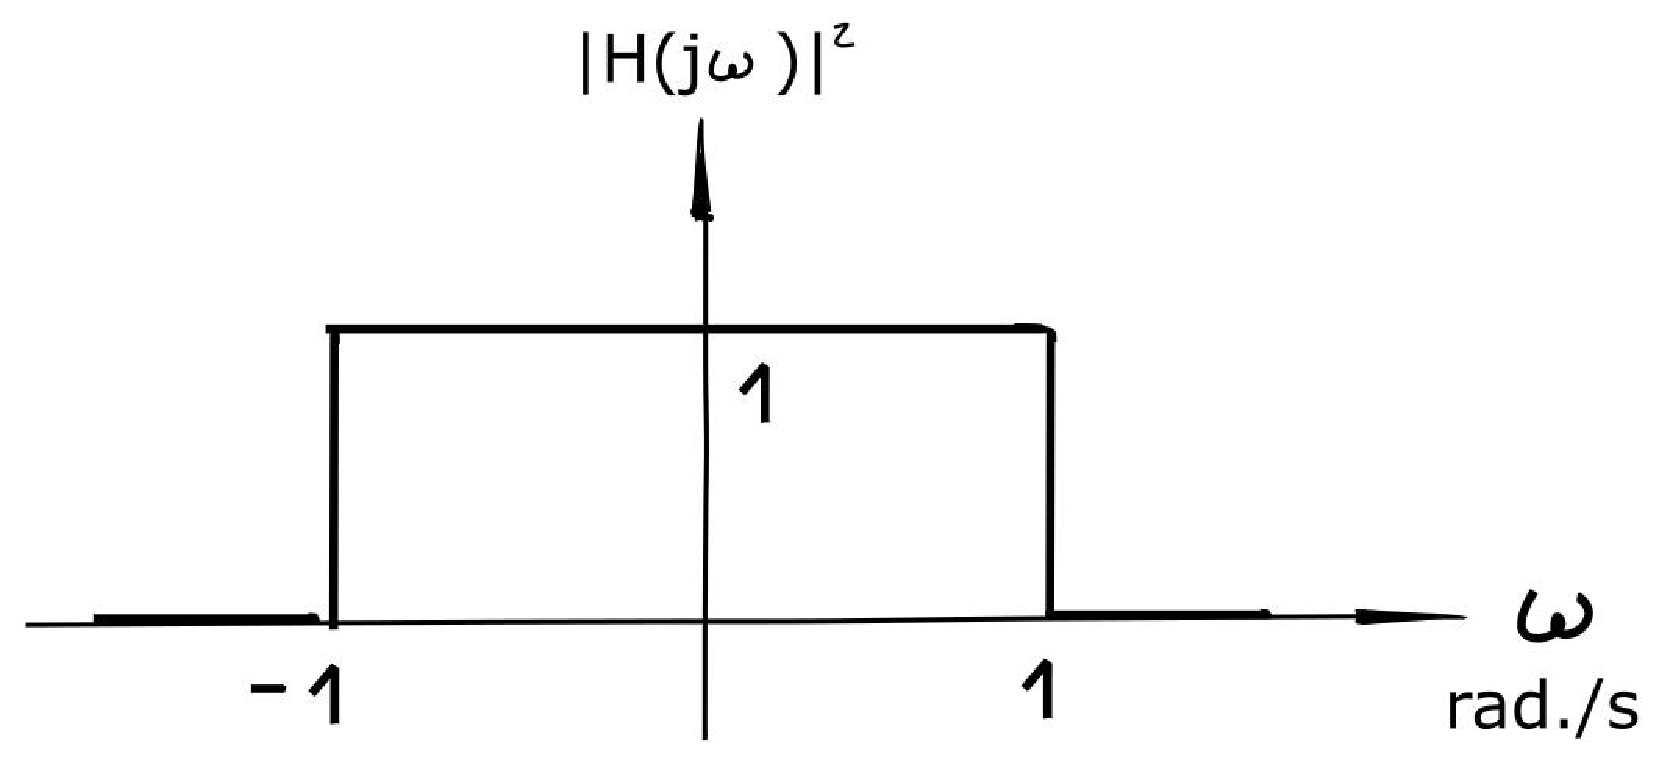
\includegraphics[scale=0.2]{filtros_ideal_funciones_magnitud.eps}
         \caption{Función de magnitud ideal}
         \label{fig:filtros:ideal:funciones:magnitud}
     \end{subfigure}
     \bigskip
     \begin{subfigure}[b]{0.5\textwidth}
         \centering
         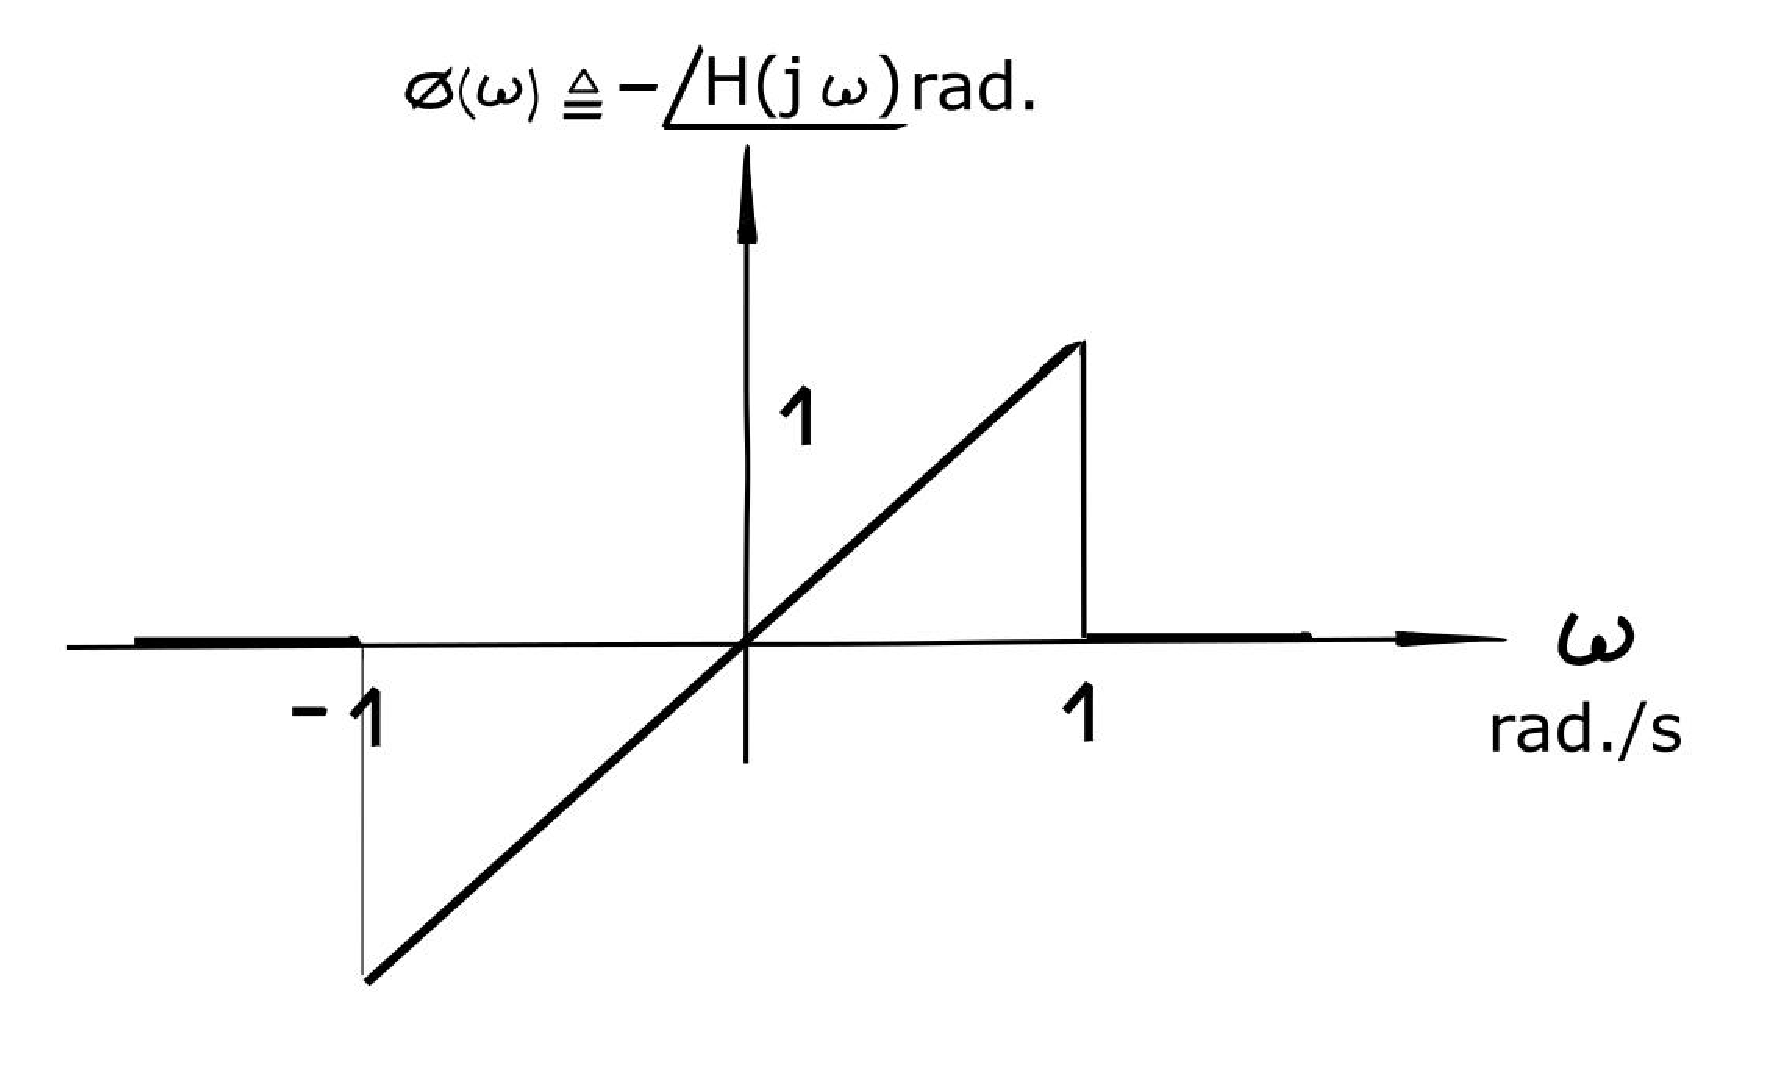
\includegraphics[scale=0.2]{filtros_ideal_funciones_fase.eps}
         \caption{Función de fase ideal}
         \label{fig:filtros:ideal:funciones:fase}
     \end{subfigure}
     \caption{Características en frecuencia de un Filtro ideal pasa bajo}
     \label{fig:filtros:ideal:funciones}
\end{figure}


Entonces, el problema de diseño radica en que ningún circuito lineal de elementos concentrados puede producir tal función de transferencia exacta. En resumen tenemos que:\newline 
1- En un filtro realizado con elementos pasivos se tiene como respuesta en frecuencia una función racional.\newline
2- Una función racional no puede tener una valor constante en ninguna banda.\newline

\textbf{ El problema de la aproximación.}\newline\newline
En la práctica se permiten ciertas tolerancias, Fig \ref{fig:filtros:funciones:tolerancia}, y esto nos lleva a que además de las bandas libres y las bandas de rechazo van a haber bandas de transición.
 
	\begin{figure}[h!]
	\centering
	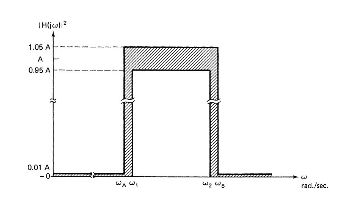
\includegraphics[scale=2.0]{funciones_tolerancia.eps}	
	\caption{Especificaciones de un filtro.}
	\label{fig:filtros:funciones:tolerancia}
	\end{figure}	 
	
De esta manera, el problema se reduce en encontrar una función $f_a(x, \alpha_1,...,\alpha_n)$ que aproxime a otra función  $f(x)$ de un filtro ideal, en un intervalo $x_1 \leq x \leq x_2$, donde los parámetros $\alpha_1$, $...$, $\alpha_n$, en la función aproximación, son encontrados por medio de algún criterio que contemple el error $\epsilon$ que surge entre la diferencia entre ambas funciones 
	$$
		\epsilon=f(x)-f_a(x; \alpha_1, ..., \alpha_n) 
	$$	

La selección de la función de aproximación se pueden dividir en los siguientes criterios.\newline

1. Mínimos cuadrados. El valor de $I(\alpha_1, ..., \alpha_2)$ definido por:
	$$
		I(\alpha_1, ..., \alpha_2) = \int_{x1}^{x2} |\epsilon|^2 w(x) dx
	$$
es minimizado, donde $w(x)$ es una función de peso, la cual atenúa el error en cierto subintervalos.\newline

2. Máxima planicidad. Las primeras $n-1$ derivadas del error, $\epsilon$, se hacen cero en $x=x_0$.\newline

3- Chebyshev. El valor de $\mu$ (constante de riple)es minimizado en el intervalo $x_1 \leq x \leq x_2$ donde $\mu=|\epsilon|_max$.\newline

4. Interpolación. Se busca que el valor del error, $\epsilon$, se reduzca para un conjunto de n puntos en el intervalo  $x_1 \leq x \leq x_2$.\newline
	
Una vez que se ha tomado alguno de estos criterio se debe determinar la forma de la función aproximación, ya sea en el dominio del tiempo o en el dominio de la frecuencia.\newline\newline

a- \underline{Selección de la función de aproximación en el dominio del tiempo}.\newline 

Consiste en aproximar una respuesta al impulso $h(t)$ desde el dominio del tiempo con una función $h^*(t)$ tal que el error sea mínimo.	
	$$
	    \epsilon = \int_{0}^{\infty}
	               { \left( h(t) - h^*(t) \right) }
 	$$
La función de aproximación va a tener la forma:
	$$
	    f_a(x; \alpha_1, ... , \alpha_n ) = \alpha_1 e^{\alpha_2 x} + \alpha_3 e^{\alpha_4 x} + ...
 	$$
Un procedimiento efectivo es usar en el dominio del tiempo funciones ortogonales, $\phi(t)$, donde la función $h^*(t)$ toma la forma
	$$
		h^*(t)=\sum_{k=1}^{n}{\alpha_k \phi_k(t)}
	$$
queda el error expresado como	
	$$
		\epsilon = 
			\int_{0}^{\infty}{ 
				\left[
					h(t) 
					-
					\sum_{k=1}^{\infty}
						{\alpha_k \phi_k(t)}
				\right]^2
						}
	$$
y es minimizado cuando
	$$
		\alpha_k = \int_{0}^{\infty}{h(t) \phi_k(t) dt} \mbox{ "      "    }  k=1,2,...,n
	$$
Si se eligen funciones ortogonales como una suma de exponenciales $e^{s_k t}$ , la respuesta al impulso será $ h^*(t)=\sum_{k=1}^{n}{\alpha_k}{ e^{s_k t} }$ y finalmente, se tendrá la transformada $H^*(s)=\sum_{k=1}^{n}{\frac{\alpha_k}{s - s_k}}$. \newline

b- \underline{Selección de la función de aproximación en el dominio del frecuencia}.\\

La selección de la función de aproximación trata en que hay que encontrar una función racional $H(s)$ que tenga alguna característica tal como máxima planicidad o igual riple. Estas características se pueden buscar en la función de magnitud, o en la función de fase. La forma de la función en general va ser
	$$
		f_a(x; \alpha_1, ... , \alpha_n) = 
		   \frac{ \alpha_1 + \alpha_3 x + \alpha_5 x^2 + ... }
		                                        { \alpha_2 + \alpha_4 x + \alpha_6 x^2 + ... }
	$$

\underline{ El filtro ideal no es realizable porque la respuesta en el impulso no es cero para $t<0$}. Por ejemplo, en el caso de buscar la máxima planicidad, la función de aproximación va a ser una función racional, donde se asume que los ceros están en infinito (filtro pasa bajos) y la función de magnitud tendrá la forma:
	$$
		M(\omega) = \frac{ K_0 }
			{ \left[1 + f(\omega^2) \right]^{1/2}}
	$$
donde $K_0$ es la constante de corriente DC ($M(j0)$) y $f(\omega^2)$ es el polinomio a ser seleccionado.\\

Por último, esta función elegida debe cumplir con los criterios de que sea realizable con elementos pasivos o elementos activos en el caso de filtros analógicos( o elementos computacionales para el caso de los filtros digitales).\\ 
\end{document}	